\documentclass[]{article}
\usepackage{graphicx}
\usepackage{hyperref}
\usepackage{amsmath}
\usepackage{caption}
\usepackage{subcaption}
\usepackage{float}


%opening
\title{VME Data Acquisition and Plastic Scintillators}
\author{Gunther T\"urk, Jonas Lehnen}

\begin{document}

\maketitle
\begin{abstract}


\end{abstract}

\tableofcontents

\newpage
\section{Theorie}
\subsection{Radiation}


\subsection{Refraction index}


\subsection{Scintillator}


\newpage
\section{Experiment}
\subsection{Setup}
This experiment we are using a long and flat plastic scintillator to detect high energetic photons or charged particles like cosmic muons. The scintillator is connected with two photo multipliers (PMT) on each side, see figure \ref{fig:setup}.

\begin{figure}[H]
\centering
\begin{subfigure}[h]{0.4\textwidth}
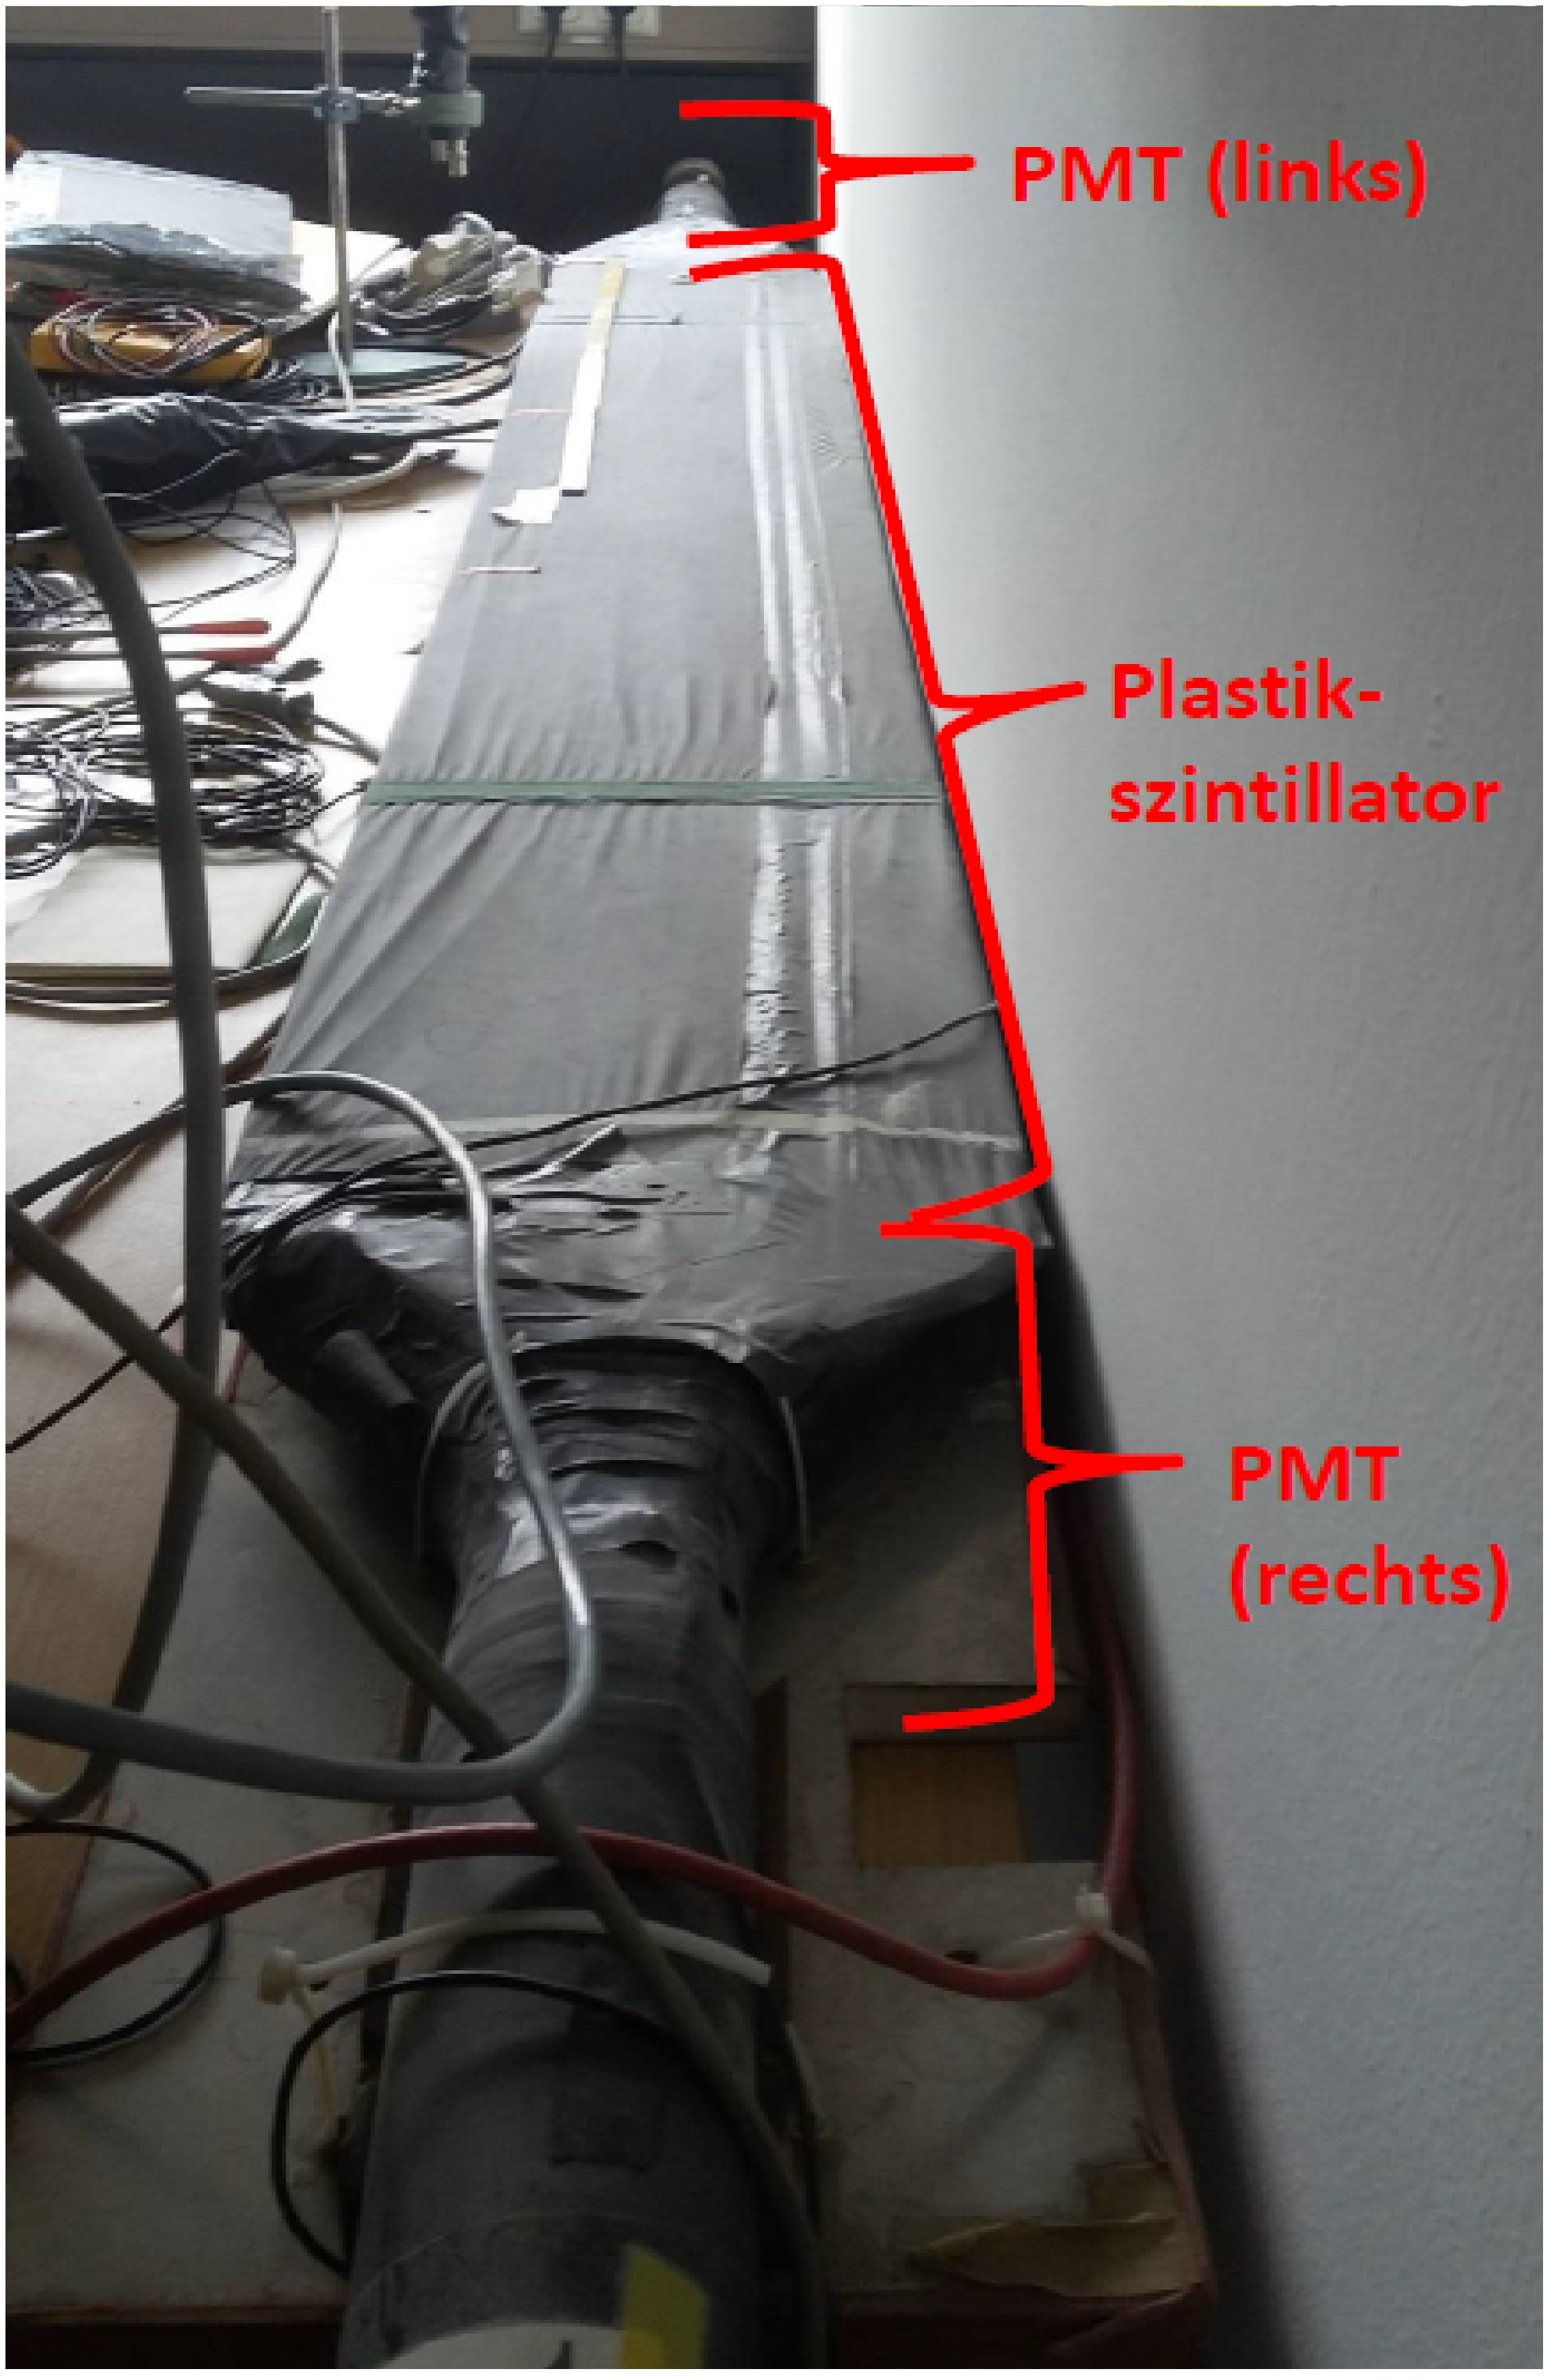
\includegraphics[width=1\textwidth]{Plots/Scintillator.jpg}
\end{subfigure}
\begin{subfigure}[h]{0.59\textwidth}
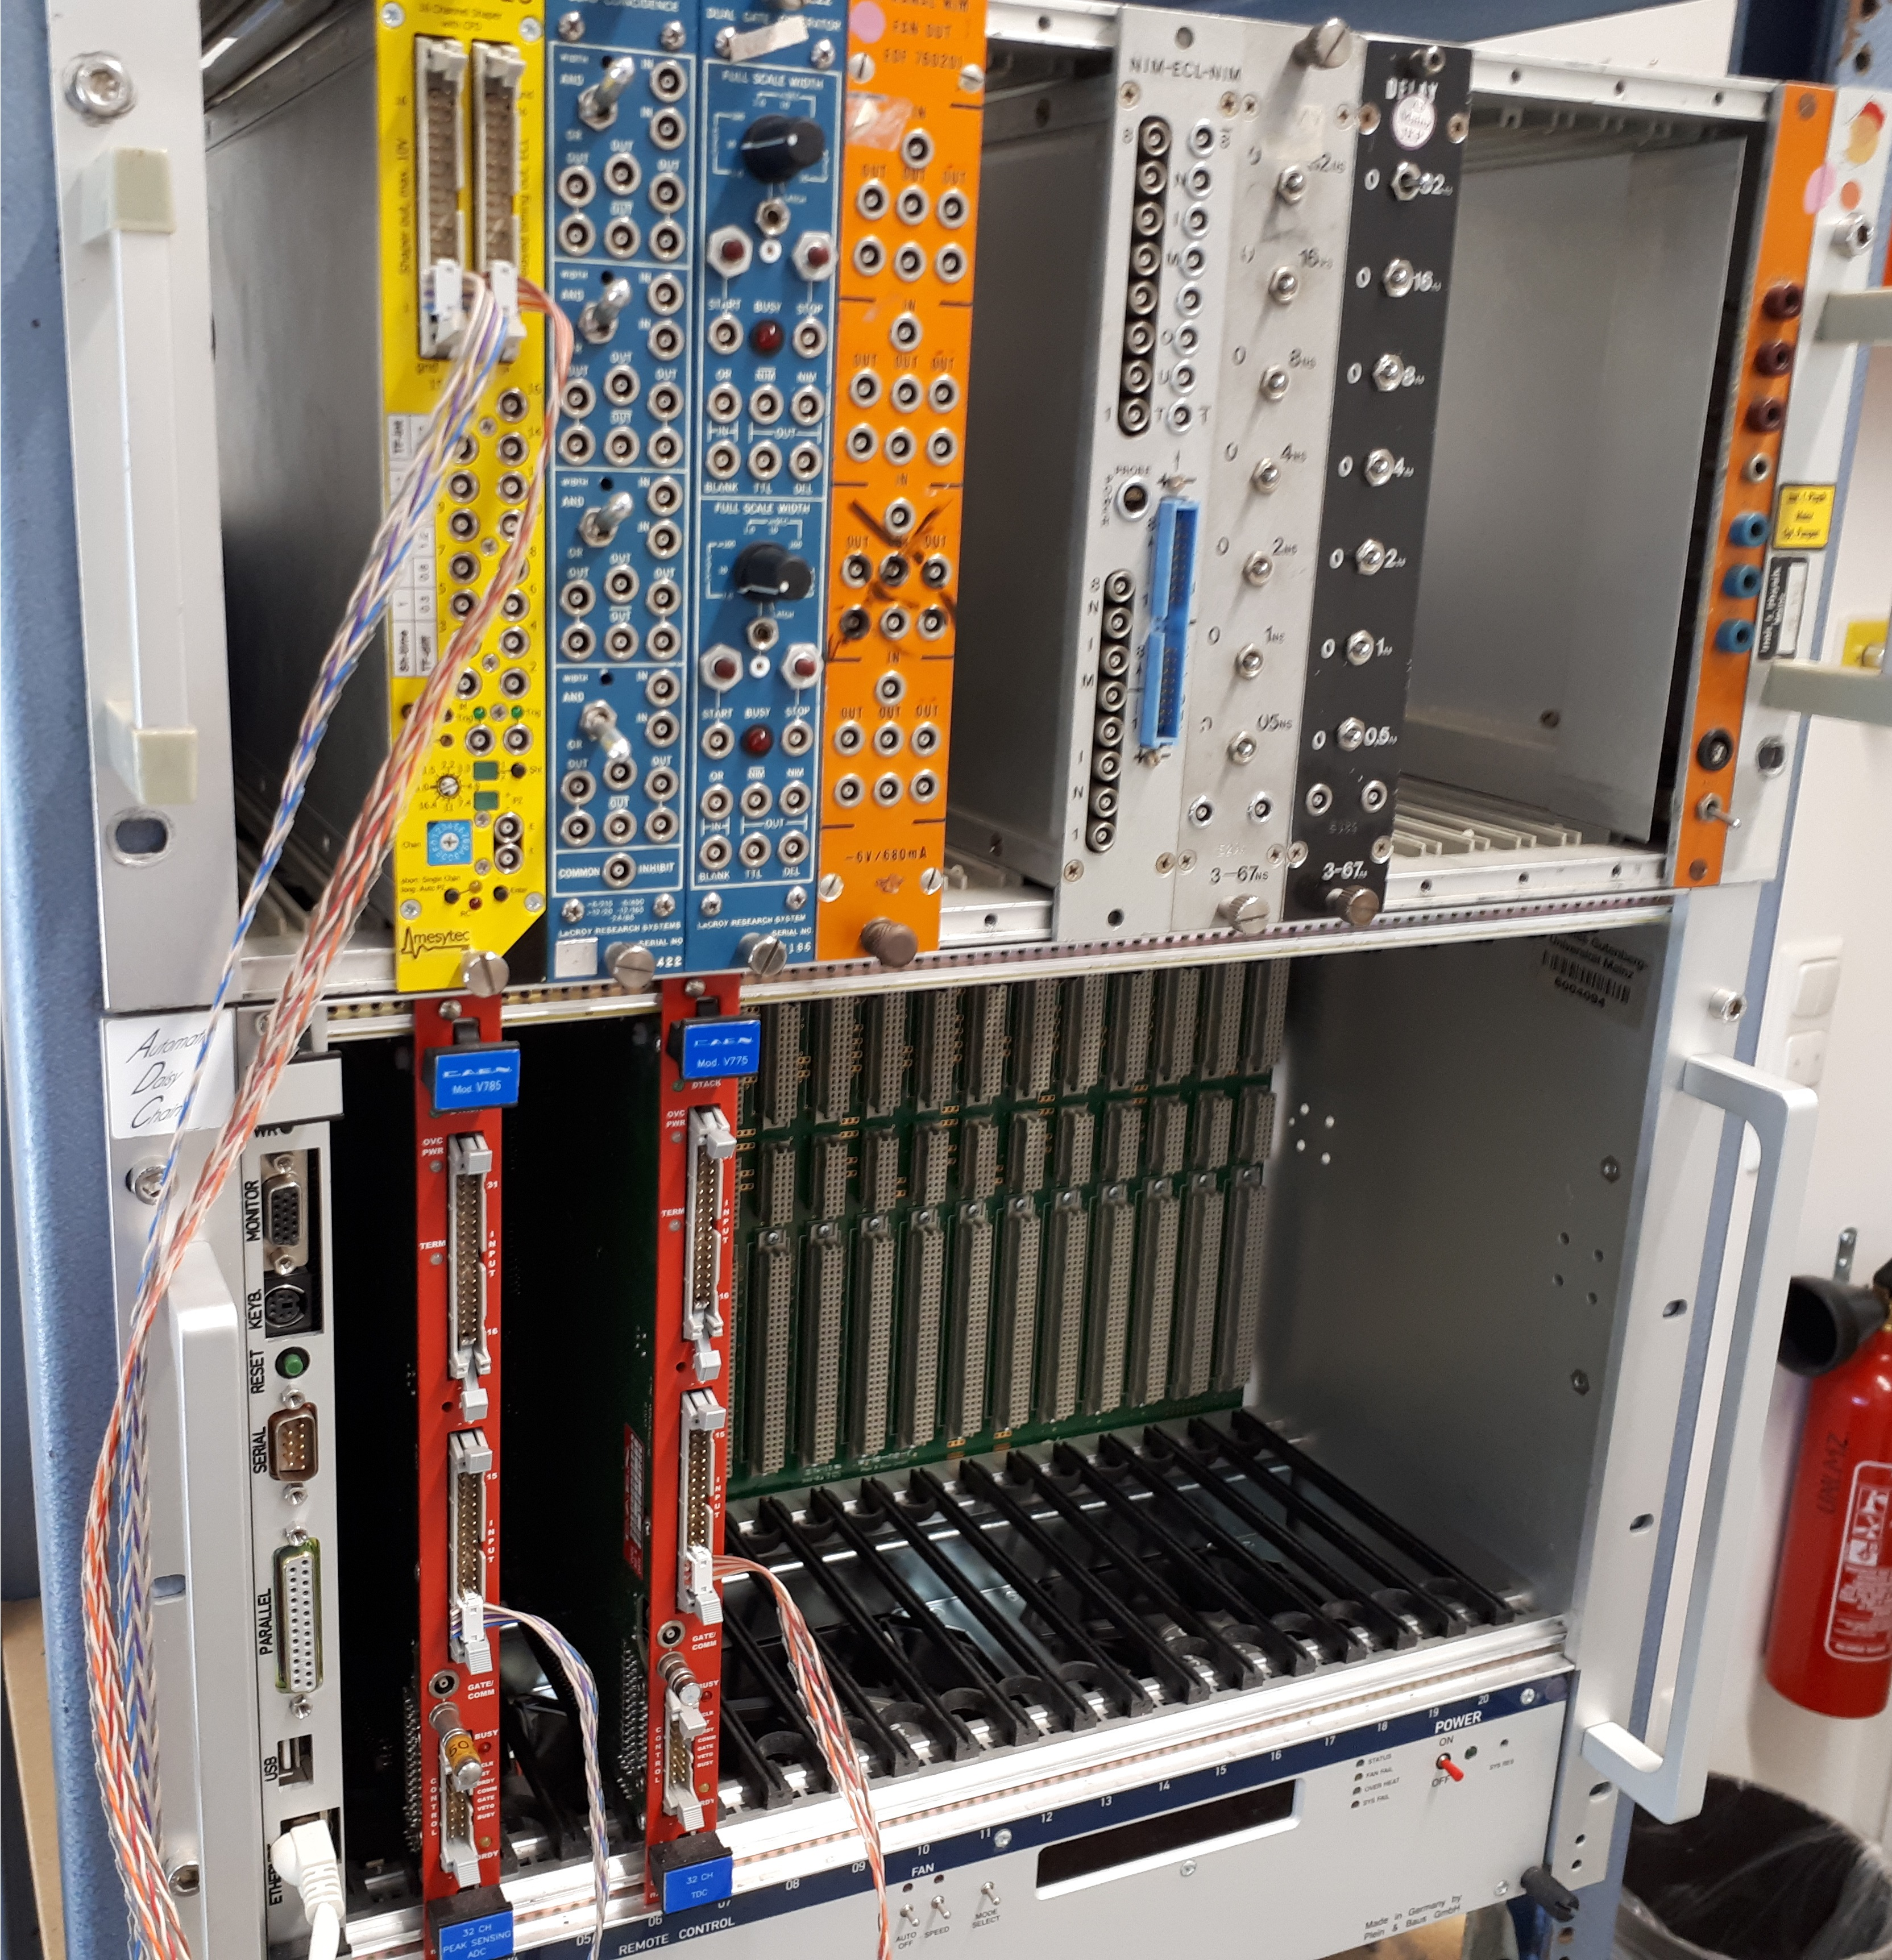
\includegraphics[width=1\textwidth]{Plots/Raw.jpg}
\end{subfigure}
\caption{Pictures of the set up. Scintillator and PMTs on the right \cite{script}. Data acquisition rack on the left without cabling. Declaration see figure \ref{fig:cabling}.}
\label{fig:setup}
\end{figure}

Both of the PMT outputs are connected with the MSCF-16 unit, the yellow one in figure \ref{fig:setup} and \ref{cabling}. The L labelled cable form the left PMT and the R labelled with an additional delay from the right one. Those Delay Boxes are just more cables the signal has to pass. From the MSCF-16 on the raw data will be delayed and passed to the analogue-to-digital converter (ADC) and time-to-digital converter (TDC) on the bottom of the pictures of the rack. And there it will be processed into the data we are working with later on. Another output leads over the third black cable to the Fan-In/-Out where the signal gets copied and passed to the Dual Gate Generator.

%%%%% Platz für mehr text :D # dont float mi floats 

\begin{figure}[H]
\centering
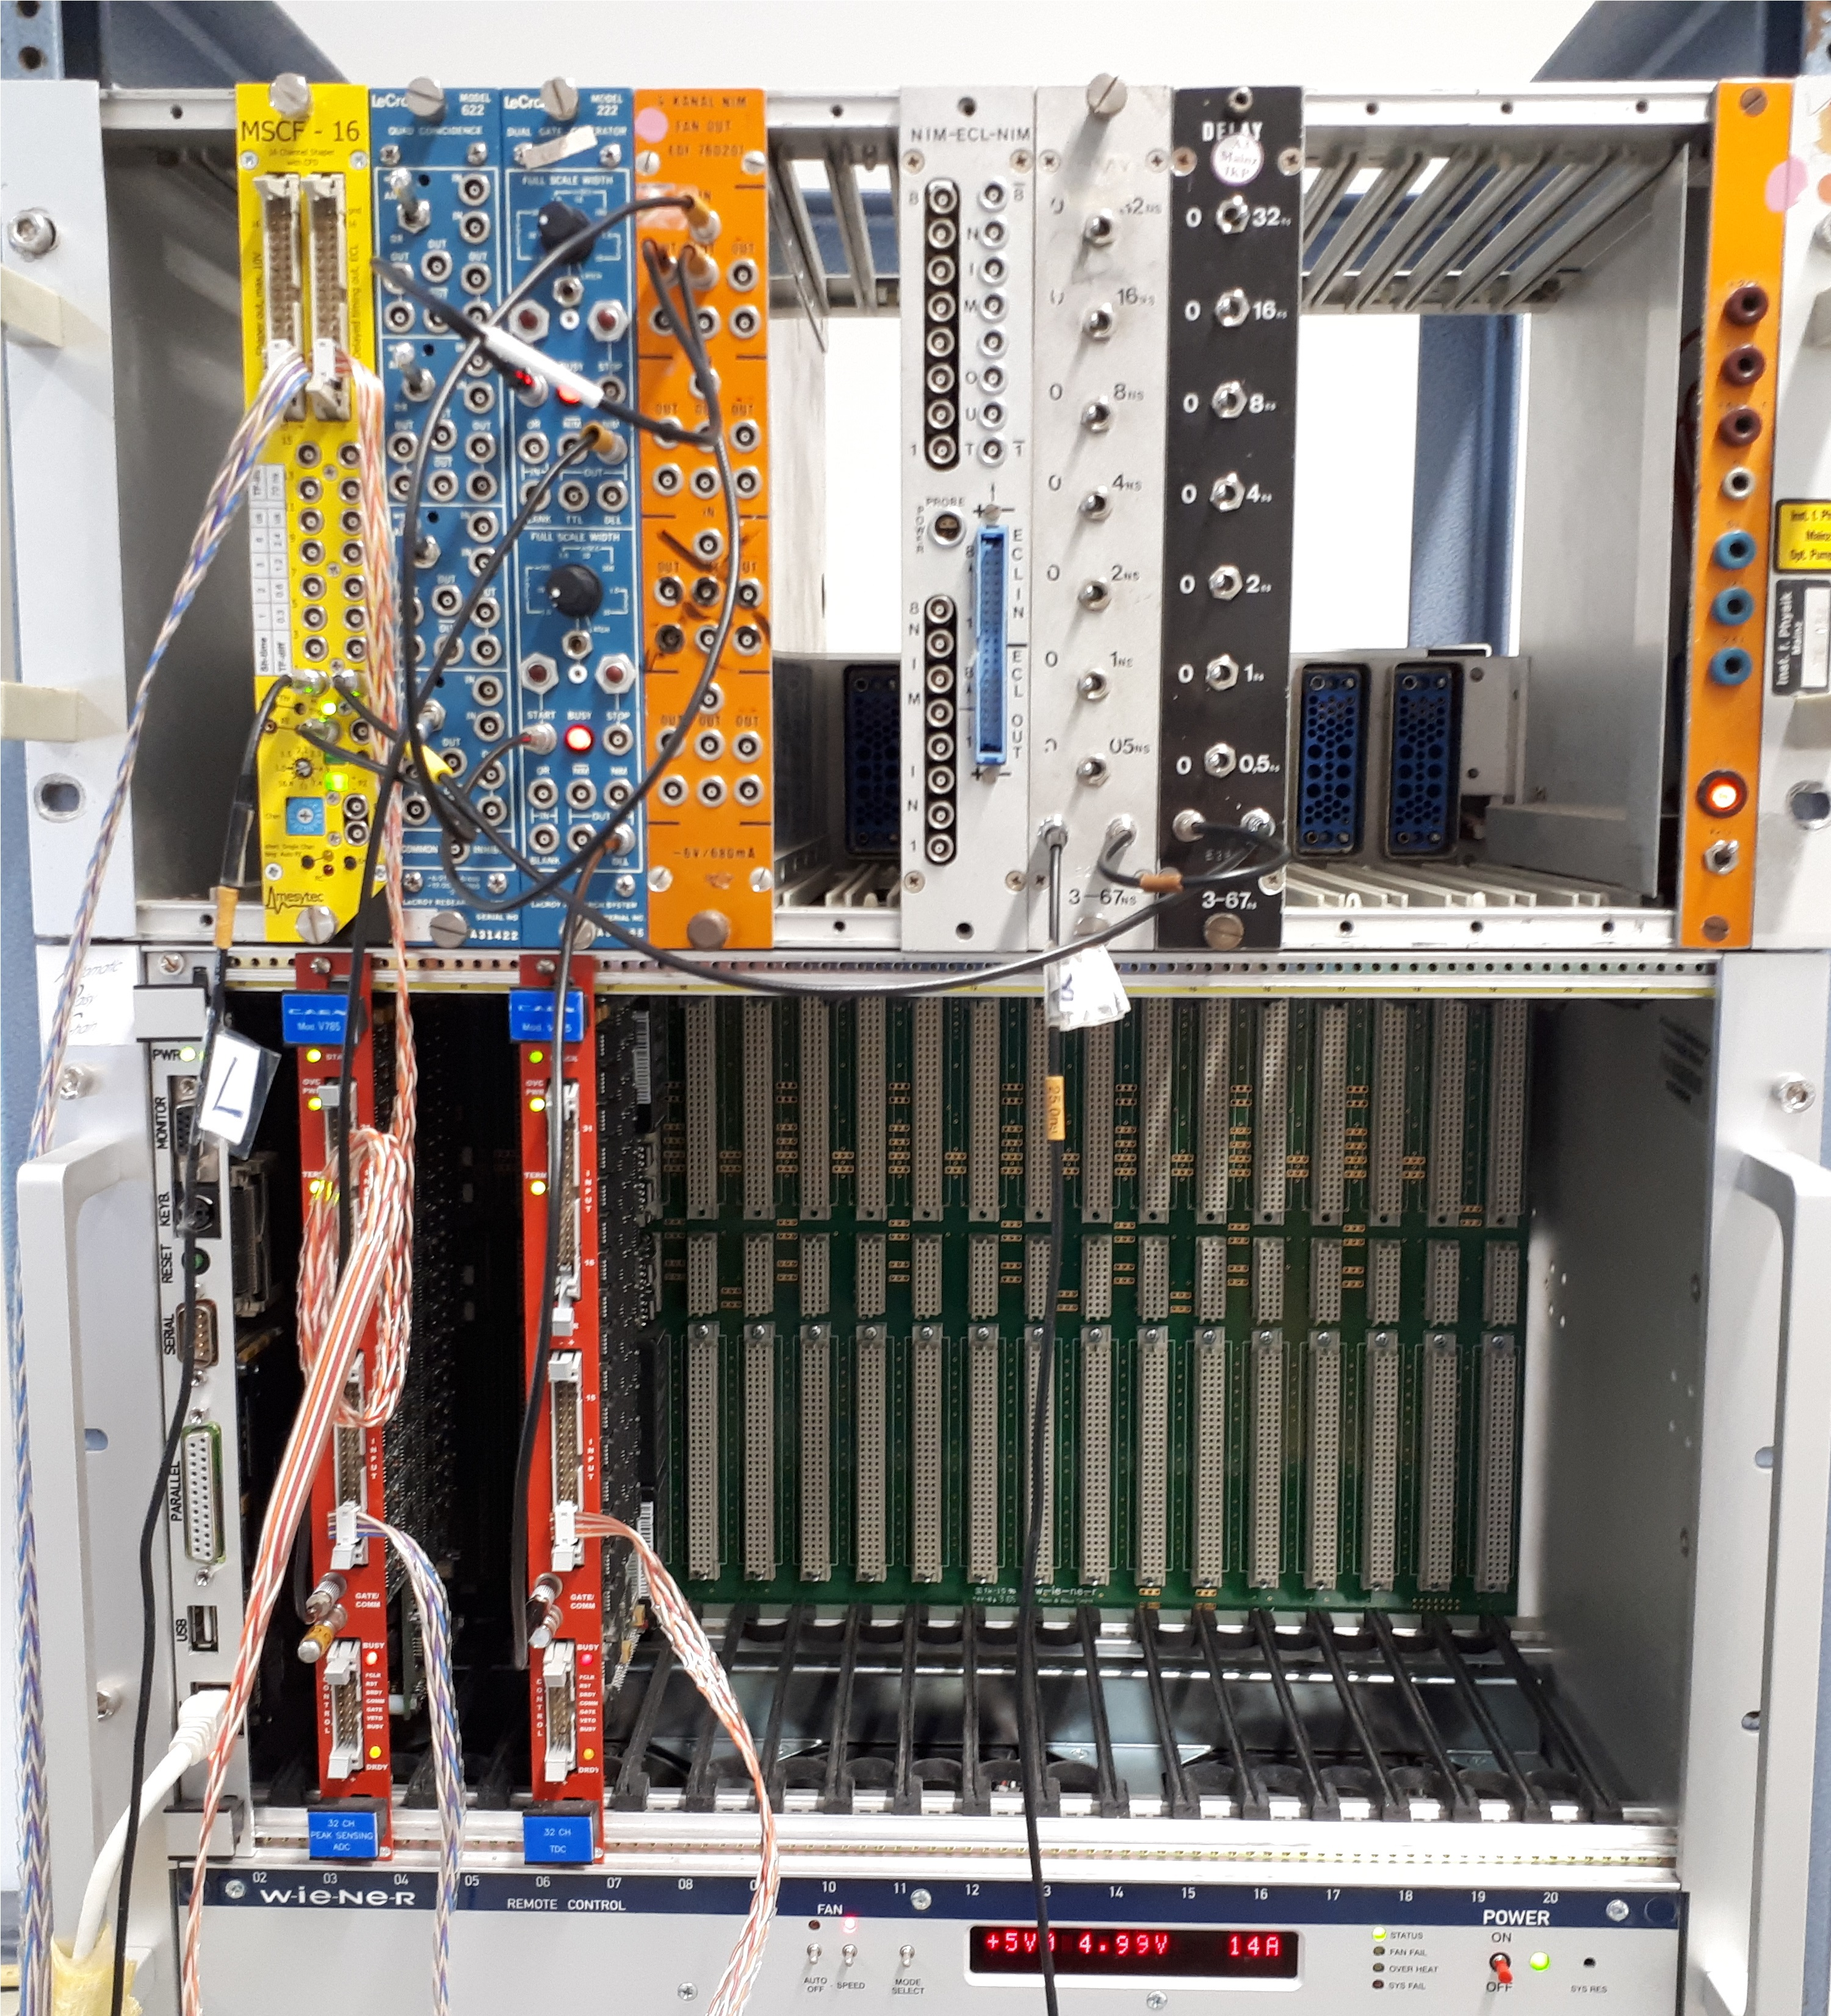
\includegraphics[width=1\textwidth]{Plots/Kabel2.jpg}
\caption{Data acquisition rack with cabling. Top left to right: MSCF-16, Quad Coincidence LeCroy 622 - not used, Dual Gate Generator LeCroy 222, Fan-In/-Out, NIM-ECL-NIM
module, two Delay Boxes.
Bottom: Gateway for PC connection, ADC, TDC.  }
\label{fig:cabling}
\end{figure}
%%%%%%%%%%%%%%%%%%%%%%%%%%%%%%%%%%%%% Kabel Schema aus Skript mit ins Bild paint'en?

The Gate Generators Delayed Output (DEL) produces a short signal for the TDC. This first signal starts the time measurement and gets stopped by the delayed signal of the MSCF-16. The length of the first triggering signal determines how long the second one will be measured. The ADC on the other hand receives a long signal from the gate generator. This leads to a good energy resolution but won't be necessary in this experiment.

%%% Description of how the data gets passed
\begin{figure}
\centering
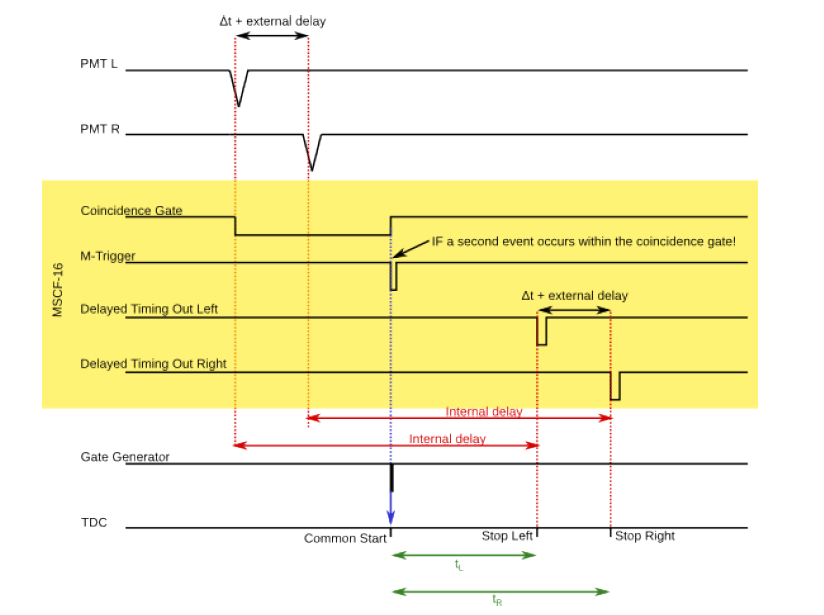
\includegraphics[width=1\textwidth]{Plots/Timing.png}
\caption{Schematic display on how the signals are passed between the components and what the TDC returns. \cite{script}}
\label{fig:timing}
\end{figure}

Now for a detailed description on what happens see figure \ref{fig:timing}. On top are the original signals the MSCF-16 receives. The signal from the right is delayed by the Delay Boxes. The first signal from the left PMT starts a coincidence gate. This is a variable time frame in which another signal has to appear to create a trigger. This helps to select 


\subsection{Cosmic Muons} % aka Setup 2.0
% Cabling via NIM_ECL_NIM to the oszi
% no photos taken
% justierung des Spannungsverteilers

\begin{figure}[H]
\centering
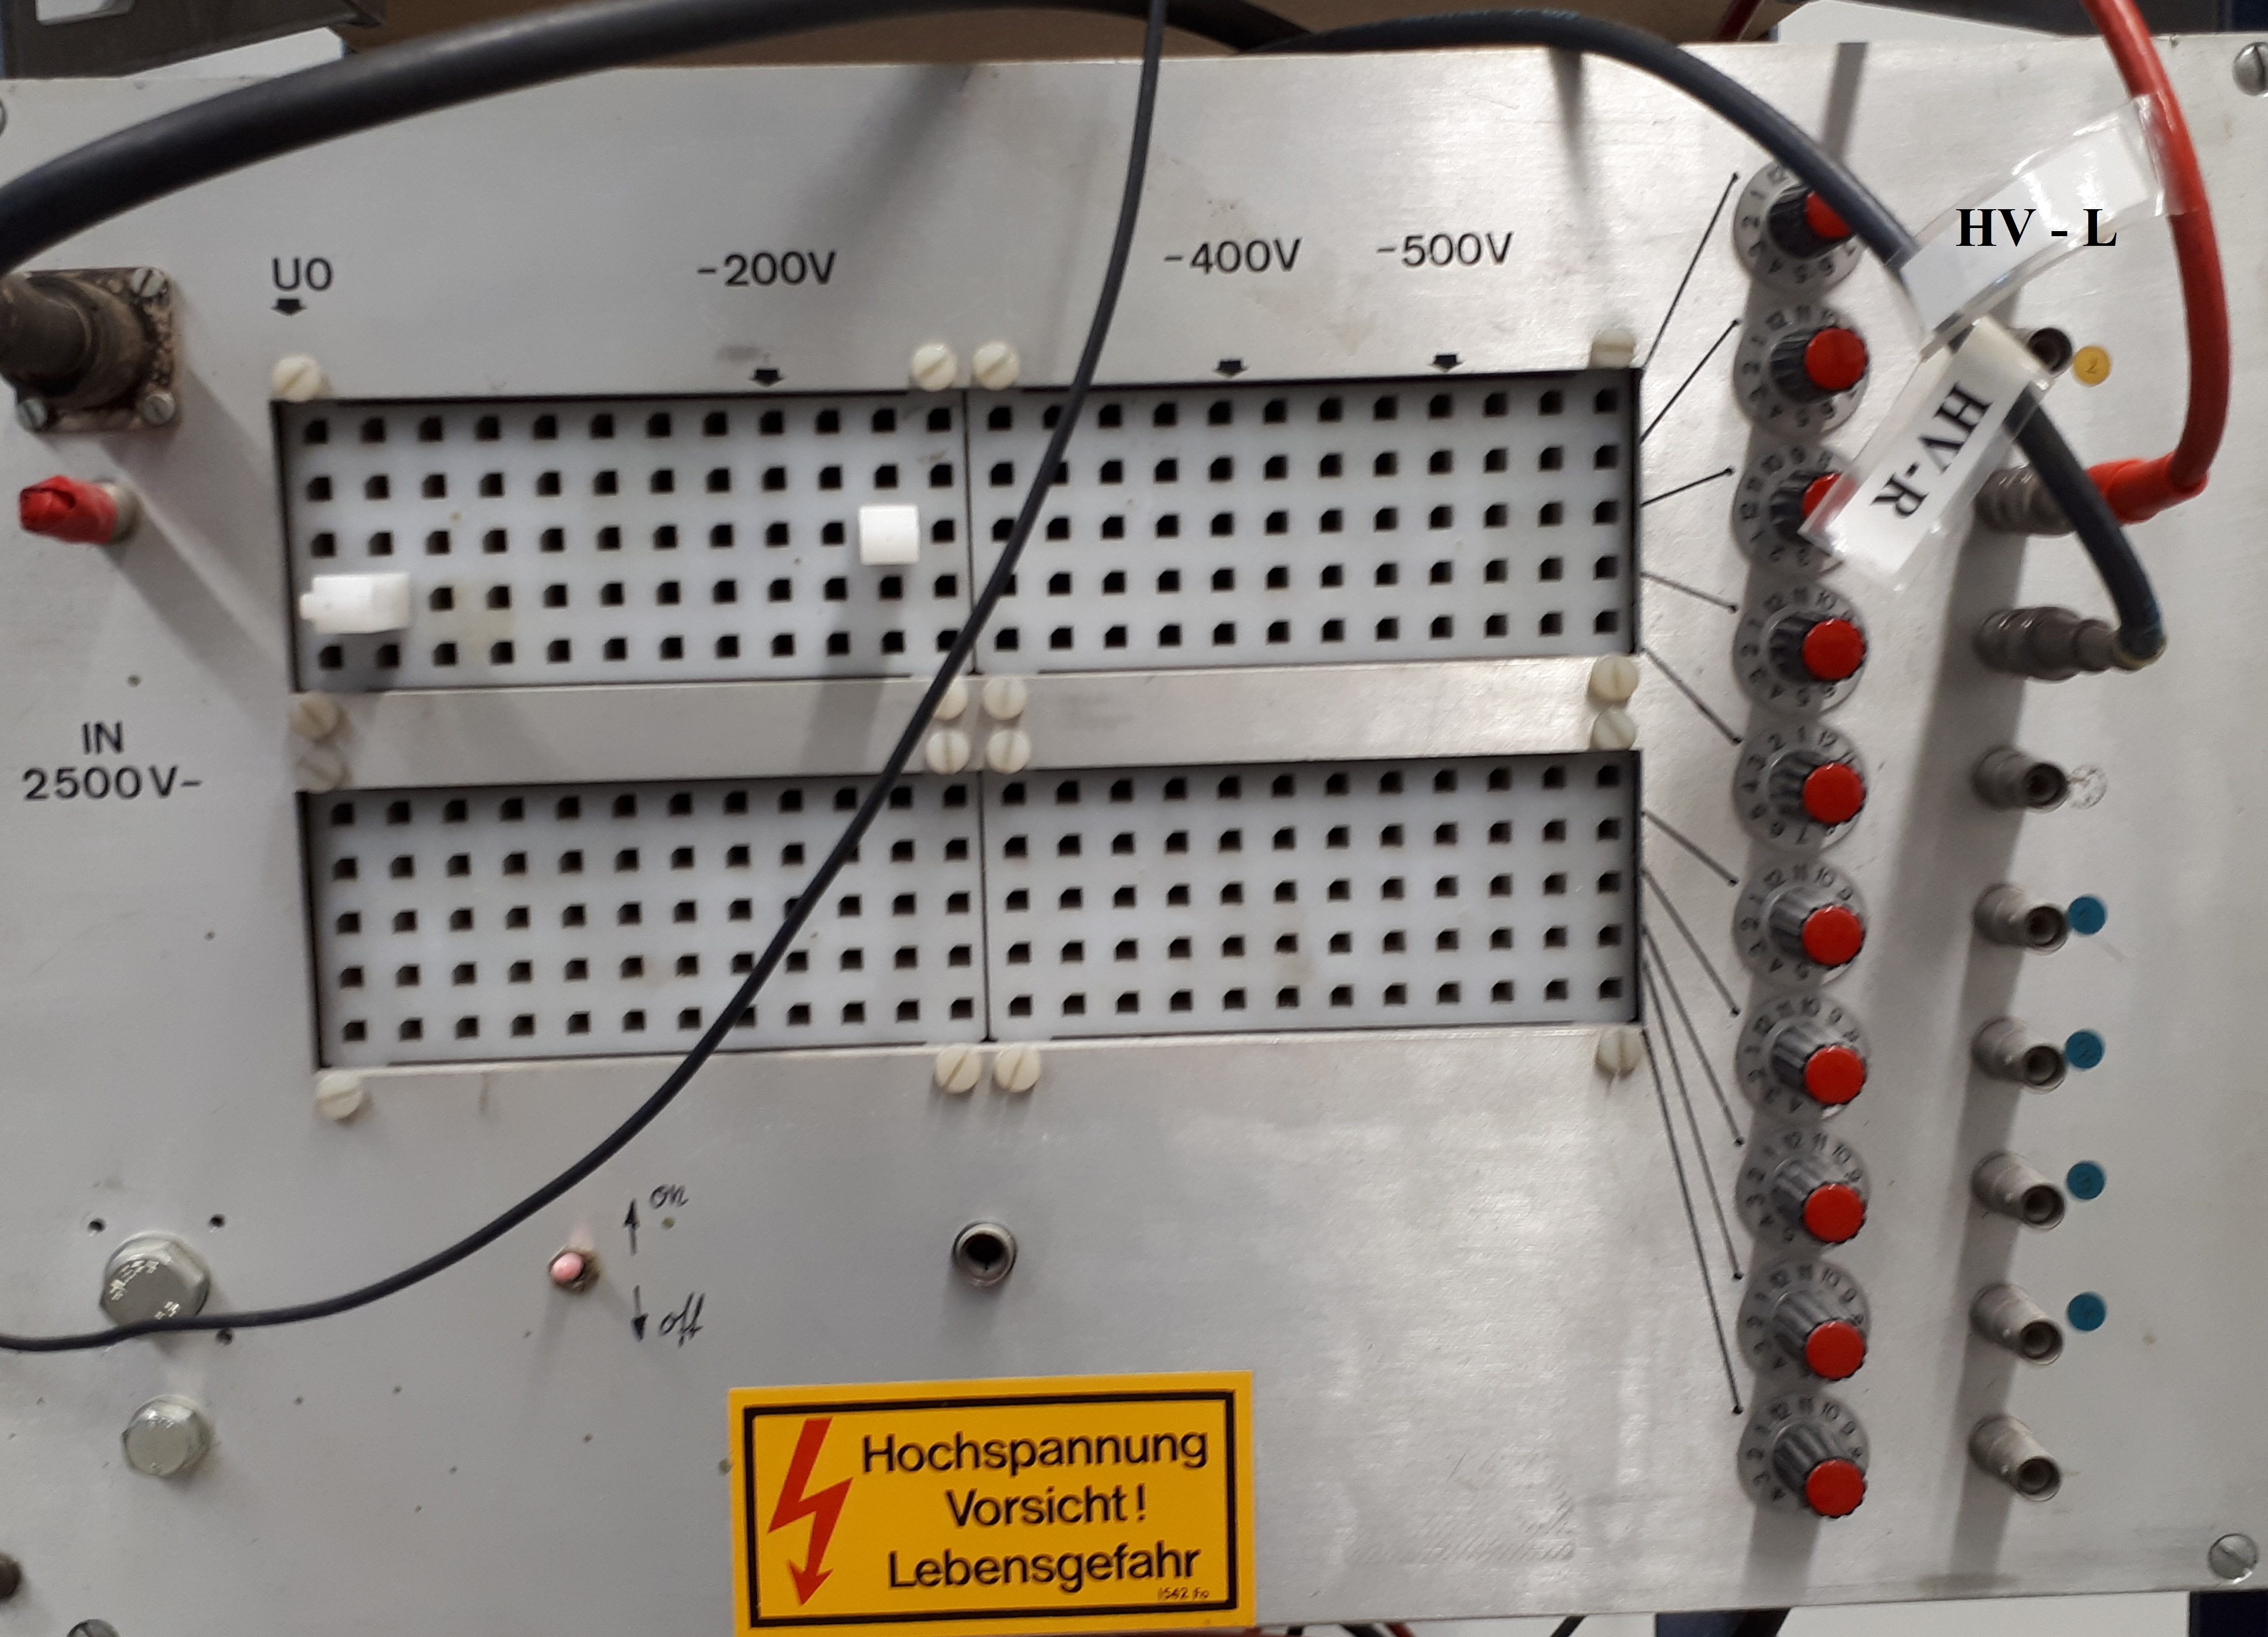
\includegraphics[width=1\textwidth]{Plots/Spannung.jpg}
\caption{Picture of the voltage distribution for similar PMT signals. HV-L (red) supplies the left PMT and HV-R (black) the right one.}
\label{fig:voltage}
\end{figure}


\subsection{Time calibration}


\subsection{Speed of light measurement}


%%% refractive index ca. 1.58 \cite{refractive index}
\section{Appendix}



\newpage
\begin{thebibliography}{}

\bibitem{script} VMEScript.pdf, script for this experiment.

\bibitem{refractive index} \begin{verbatim}
https://eljentechnology.com/images/products/data_sheets/
  EJ-228_EJ-230.pdf
 https://www.crystals.saint-gobain.com/sites/imdf.crystals.com/
  files/documents/sgc-bc400-404-408-412-416-data-sheet.pdf
\end{verbatim} 


\end{thebibliography}
\end{document}

